\documentclass[aspectratio=169]{beamer}
\usetheme{metropolis}
\usepackage{amsmath}
\usepackage{graphicx}
\usepackage{tikz}
\usepackage{booktabs}

\title{Finite Difference Methods for Black-Scholes - Part 1}
\subtitle{Introduction and Explicit Method}
\author{Lecturer}
\date{\today}

\begin{document}

\begin{frame}
\titlepage
\end{frame}

\begin{frame}
\frametitle{Outline - Part 1}
\tableofcontents
\end{frame}

\section{Introduction and Main Example}

\begin{frame}
\frametitle{The Black-Scholes PDE}
The Black-Scholes equation for option pricing is:

\[\frac{\partial V}{\partial t} + \frac{1}{2}\sigma^2 S^2 \frac{\partial^2 V}{\partial S^2} + rS \frac{\partial V}{\partial S} - rV = 0\]

This parabolic PDE describes how option values evolve over time.
\end{frame}

\begin{frame}
\frametitle{Why Use Numerical Methods?}
\begin{itemize}
\item Analytical solutions exist for simple cases (European options)
\item Complex options require numerical methods
\item Finite difference methods are powerful numerical techniques
\item Allow pricing of exotic and path-dependent options
\end{itemize}
\end{frame}

\begin{frame}
\frametitle{Our Main Example: European Call Option}
Throughout this presentation, we'll solve the same example:

\begin{block}{Example Parameters}
\begin{itemize}
\item \textbf{Option type}: European call option
\item \textbf{Current stock price}: $S_0 = 100$
\item \textbf{Strike price}: $K = 100$
\item \textbf{Time to expiration}: $T = 0.25$ years (3 months)
\end{itemize}
\end{block}
\end{frame}

\begin{frame}
\frametitle{Example Parameters (continued)}
\begin{block}{Market Parameters}
\begin{itemize}
\item \textbf{Risk-free rate}: $r = 0.05$ (5\% per annum)
\item \textbf{Volatility}: $\sigma = 0.2$ (20\% per annum)
\end{itemize}
\end{block}

\textbf{Goal}: Find the option value $V(100, 0)$ at current time

\begin{block}{Analytical Benchmark}
Black-Scholes formula gives: $V_{\text{BS}} = 4.61$
\end{block}
\end{frame}

\section{Black-Scholes Analytical Benchmark}

\begin{frame}
\frametitle{Black-Scholes Formula for European Call Options}
The analytical Black-Scholes formula provides our benchmark:

\begin{block}{Black-Scholes Formula}
\[V = S_0 \times N(d_1) - K \times e^{-r \times T} \times N(d_2)\]
\end{block}

Where:
\begin{itemize}
\item $N(x)$ = cumulative standard normal distribution function
\item $d_1$ and $d_2$ are calculated using specific formulas
\end{itemize}
\end{frame}

\begin{frame}
\frametitle{Calculating $d_1$ and $d_2$}
\begin{block}{The $d_1$ and $d_2$ Parameters}
\begin{align}
d_1 &= \frac{\ln(S_0/K) + (r + \sigma^2/2) \times T}{\sigma \times \sqrt{T}} \\
d_2 &= d_1 - \sigma \times \sqrt{T}
\end{align}
\end{block}

These parameters capture:
\begin{itemize}
\item \textbf{$d_1$}: Measures "moneyness" adjusted for time and volatility
\item \textbf{$d_2$}: Adjusts $d_1$ for the volatility effect over time
\end{itemize}
\end{frame}

\begin{frame}
\frametitle{Step 1: Calculate $d_1$}
Using our example parameters:
\begin{itemize}
\item $S_0 = 100$, $K = 100$, $T = 0.25$, $r = 0.05$, $\sigma = 0.2$
\end{itemize}

\begin{align}
d_1 &= \frac{\ln(100/100) + (0.05 + 0.2^2/2) \times 0.25}{0.2 \times \sqrt{0.25}} \\
&= \frac{0 + (0.05 + 0.02) \times 0.25}{0.2 \times 0.5} \\
&= \frac{0.0175}{0.1} = 0.175
\end{align}
\end{frame}

\begin{frame}
\frametitle{Step 2: Calculate $d_2$}
\begin{align}
d_2 &= d_1 - \sigma \times \sqrt{T} \\
&= 0.175 - 0.2 \times \sqrt{0.25} \\
&= 0.175 - 0.2 \times 0.5 \\
&= 0.175 - 0.1 = 0.075
\end{align}
\end{frame}

\begin{frame}
\frametitle{Step 3: Normal Distribution Values}
We need to find the cumulative standard normal distribution values:

\begin{block}{Normal Distribution Evaluations}
\begin{itemize}
\item $N(d_1) = N(0.175) \approx 0.5695$
\item $N(d_2) = N(0.075) \approx 0.5299$
\end{itemize}
\end{block}

\textbf{Note}: These values can be found using:
\begin{itemize}
\item Statistical tables
\item Financial calculators
\item Software functions (Excel NORMSDIST, Python scipy.stats.norm.cdf)
\end{itemize}
\end{frame}

\begin{frame}
\frametitle{Step 4: Apply the Black-Scholes Formula}
\begin{align}
V &= S_0 \times N(d_1) - K \times e^{-r \times T} \times N(d_2) \\
&= 100 \times 0.5695 - 100 \times e^{-0.05 \times 0.25} \times 0.5299 \\
&= 56.95 - 100 \times 0.9876 \times 0.5299 \\
&= 56.95 - 52.33 = 4.62
\end{align}

\textbf{Note}: With higher precision calculations, the exact result is $V_{BS} = 4.61$
\end{frame}

\begin{frame}
\frametitle{Understanding the Black-Scholes Components}
\begin{block}{Economic Interpretation}
\begin{itemize}
\item \textbf{$S_0 \times N(d_1)$}: Expected value of stock if option is exercised
\item \textbf{$K \times e^{-rT} \times N(d_2)$}: Present value of strike price, weighted by exercise probability
\item \textbf{$N(d_1)$, $N(d_2)$}: Risk-adjusted probabilities related to option finishing in-the-money
\end{itemize}
\end{block}

This analytical solution serves as our benchmark for numerical methods!
\end{frame}

\section{Numerical Method Setup}

\begin{frame}
\frametitle{Grid Setup - Domain}
\textbf{Computational domain:}

\begin{itemize}
\item \textbf{Price range}: $[0, 200]$ with $S_{\max} = 200$
\item \textbf{Time range}: $[0, 0.25]$ years
\end{itemize}
\end{frame}

\begin{frame}
\frametitle{Grid Setup - Discretization}
\textbf{Grid discretization:}

\begin{itemize}
\item \textbf{Price steps}: $M = 20$ intervals, $\Delta S = 10$
\item \textbf{Time steps}: $N = 25$ intervals, $\Delta t = 0.01$
\item \textbf{Grid points}: $S_i = i \cdot 10$ for $i = 0, 1, ..., 20$
\item \textbf{Time points}: $t_j = j \cdot 0.01$ for $j = 0, 1, ..., 25$
\end{itemize}
\end{frame}

\begin{frame}
\frametitle{Grid Visualization}
\begin{center}
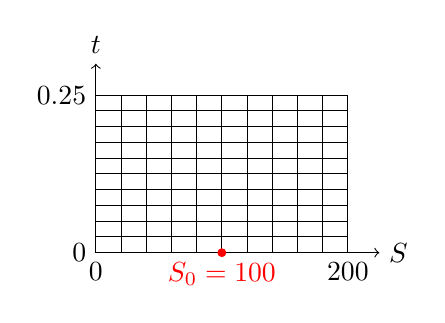
\begin{tikzpicture}[scale=0.8]
\draw[->] (0,0) -- (4.5,0) node[right] {$S$};
\draw[->] (0,0) -- (0,3) node[above] {$t$};
\foreach \x in {0,0.4,0.8,1.2,1.6,2.0,2.4,2.8,3.2,3.6,4.0} {
  \draw (\x,0) -- (\x,2.5);
}
\foreach \y in {0,0.25,0.5,0.75,1.0,1.25,1.5,1.75,2.0,2.25,2.5} {
  \draw (0,\y) -- (4,\y);
}
\node[below] at (0,0) {$0$};
\node[below] at (4,0) {$200$};
\node[left] at (0,0) {$0$};
\node[left] at (0,2.5) {$0.25$};
% Mark our point of interest
\fill[red] (2,0) circle (2pt);
\node[below, red] at (2,0) {$S_0=100$};
\end{tikzpicture}
\end{center}
\end{frame}

\begin{frame}
\frametitle{Boundary Conditions}
\begin{block}{Terminal Condition (at expiration)}
$V(S_i, 0.25) = \max(S_i - 100, 0)$
\end{block}

\begin{block}{Spatial Boundaries}
\begin{itemize}
\item \textbf{At $S = 0$}: $V(0, t) = 0$
\item \textbf{At $S = 200$}: $V(200, t) = 200 - 100e^{-0.05(0.25-t)}$
\end{itemize}
\end{block}
\end{frame}

\section{Finite Difference Discretization Fundamentals}

\begin{frame}
\frametitle{Why Do We Need Discretization?}
\textbf{The Challenge}:
\begin{itemize}
\item PDEs involve continuous derivatives
\item Computers work with discrete values
\item Need to approximate derivatives using grid points
\end{itemize}

\textbf{Our Goal}:
Replace $\frac{\partial V}{\partial S}$ and $\frac{\partial^2 V}{\partial S^2}$ with discrete approximations
\end{frame}

\begin{frame}
\frametitle{Forward Difference Approximation}
\textbf{Basic Idea}: Use the current point and the next point

\begin{block}{Forward Difference Formula}
\[\frac{\partial V}{\partial S} \bigg|_{i,j} \approx \frac{V_{i+1,j} - V_{i,j}}{\Delta S}\]
\end{block}

\textbf{Properties}:
\begin{itemize}
\item Accuracy: $O(\Delta S)$ - first order
\item Uses "future" information (point $i+1$)
\item Simple to implement
\end{itemize}
\end{frame}

\begin{frame}
\frametitle{Backward Difference Approximation}
\textbf{Basic Idea}: Use the current point and the previous point

\begin{block}{Backward Difference Formula}
\[\frac{\partial V}{\partial S} \bigg|_{i,j} \approx \frac{V_{i,j} - V_{i-1,j}}{\Delta S}\]
\end{block}

\textbf{Properties}:
\begin{itemize}
\item Accuracy: $O(\Delta S)$ - first order
\item Uses "past" information (point $i-1$)
\item More stable than forward difference
\end{itemize}
\end{frame}

\begin{frame}
\frametitle{Central Difference Approximation}
\textbf{Basic Idea}: Use points on both sides of current point

\begin{block}{Central Difference Formula}
\[\frac{\partial V}{\partial S} \bigg|_{i,j} \approx \frac{V_{i+1,j} - V_{i-1,j}}{2\Delta S}\]
\end{block}

\textbf{Properties}:
\begin{itemize}
\item Accuracy: $O((\Delta S)^2)$ - second order!
\item More accurate than forward/backward
\item Most commonly used for spatial derivatives
\end{itemize}
\end{frame}

\begin{frame}
\frametitle{Why is Central Difference More Accurate?}
\textbf{Taylor Expansion Analysis}:

Around point $i$:
\begin{align}
V_{i+1,j} &= V_{i,j} + \Delta S \frac{\partial V}{\partial S} + \frac{(\Delta S)^2}{2} \frac{\partial^2 V}{\partial S^2} + O((\Delta S)^3) \\
V_{i-1,j} &= V_{i,j} - \Delta S \frac{\partial V}{\partial S} + \frac{(\Delta S)^2}{2} \frac{\partial^2 V}{\partial S^2} + O((\Delta S)^3)
\end{align}

\textbf{Key Insight}: When we subtract these equations, the second-derivative terms cancel out!
\end{frame}

\begin{frame}
\frametitle{Central Difference Derivation}
Subtracting the Taylor expansions:
\[V_{i+1,j} - V_{i-1,j} = 2\Delta S \frac{\partial V}{\partial S} + O((\Delta S)^3)\]

Solving for the derivative:
\[\frac{\partial V}{\partial S} = \frac{V_{i+1,j} - V_{i-1,j}}{2\Delta S} + O((\Delta S)^2)\]

\textbf{Result}: Error is $O((\Delta S)^2)$ instead of $O(\Delta S)$
\end{frame}

\begin{frame}
\frametitle{Second Derivative Approximation}
\textbf{Goal}: Approximate $\frac{\partial^2 V}{\partial S^2}$

\begin{block}{Central Difference for Second Derivative}
\[\frac{\partial^2 V}{\partial S^2} \bigg|_{i,j} \approx \frac{V_{i+1,j} - 2V_{i,j} + V_{i-1,j}}{(\Delta S)^2}\]
\end{block}

\textbf{Accuracy}: $O((\Delta S)^2)$ - second order
\end{frame}

\begin{frame}
\frametitle{Second Derivative Derivation}
Adding the Taylor expansions:
\[V_{i+1,j} + V_{i-1,j} = 2V_{i,j} + (\Delta S)^2 \frac{\partial^2 V}{\partial S^2} + O((\Delta S)^4)\]

Rearranging:
\[\frac{\partial^2 V}{\partial S^2} = \frac{V_{i+1,j} - 2V_{i,j} + V_{i-1,j}}{(\Delta S)^2} + O((\Delta S)^2)\]

\textbf{Note}: The first derivative terms cancel out automatically!
\end{frame}

\begin{frame}
\frametitle{Time Derivative - Forward Difference}
\textbf{For Explicit Methods}:

\begin{block}{Forward Difference in Time}
\[\frac{\partial V}{\partial t} \bigg|_{i,j} \approx \frac{V_{i,j+1} - V_{i,j}}{\Delta t}\]
\end{block}

\begin{itemize}
\item Uses known values at time $j$ to find values at time $j+1$
\item Creates explicit update formulas
\item Accuracy: $O(\Delta t)$
\end{itemize}
\end{frame}

\begin{frame}
\frametitle{Time Derivative - Backward Difference}
\textbf{For Implicit Methods}:

\begin{block}{Backward Difference in Time}
\[\frac{\partial V}{\partial t} \bigg|_{i,j+1} \approx \frac{V_{i,j+1} - V_{i,j}}{\Delta t}\]
\end{block}

\begin{itemize}
\item Uses unknown values at time $j+1$ in the equation
\item Creates systems of equations to solve
\item Accuracy: $O(\Delta t)$
\end{itemize}
\end{frame}

\begin{frame}
\frametitle{Time Derivative - Central Difference}
\textbf{For Crank-Nicolson Method}:

\begin{block}{Central Difference in Time}
\[\frac{\partial V}{\partial t} \bigg|_{i,j+1/2} \approx \frac{V_{i,j+1} - V_{i,j}}{\Delta t}\]
\end{block}

\begin{itemize}
\item Evaluates spatial operators at both time levels
\item Averages explicit and implicit approaches
\item Accuracy: $O((\Delta t)^2)$ - second order!
\end{itemize}
\end{frame}

\begin{frame}
\frametitle{Accuracy Comparison}
\begin{center}
\begin{tabular}{lcc}
\toprule
\textbf{Method} & \textbf{Formula} & \textbf{Accuracy} \\
\midrule
Forward & $\frac{V_{i+1} - V_i}{\Delta S}$ & $O(\Delta S)$ \\
Backward & $\frac{V_i - V_{i-1}}{\Delta S}$ & $O(\Delta S)$ \\
Central & $\frac{V_{i+1} - V_{i-1}}{2\Delta S}$ & $O((\Delta S)^2)$ \\
\bottomrule
\end{tabular}
\end{center}

\textbf{Key Takeaway}: Central differences are more accurate!
\end{frame}

\begin{frame}
\frametitle{Grid Requirements}
\textbf{Boundary Issues}:
\begin{itemize}
\item Forward difference: Can't use at rightmost point
\item Backward difference: Can't use at leftmost point  
\item Central difference: Can't use at either boundary
\end{itemize}

\textbf{Solution}: Use different approximations near boundaries or impose boundary conditions
\end{frame}

\section{Explicit Finite Difference Method}

\begin{frame}
\frametitle{Explicit Method - Basic Idea}
Replace derivatives with finite difference approximations using known values at current time level.

\begin{block}{Key Concept}
Use values at time $j$ to compute values at time $j+1$
\end{block}
\end{frame}

\begin{frame}
\frametitle{Explicit Method - Discretization}
\begin{block}{Discretized Black-Scholes Equation}
\[\frac{V_{i,j+1} - V_{i,j}}{\Delta t} + \frac{1}{2}\sigma^2 S_i^2 \frac{V_{i+1,j} - 2V_{i,j} + V_{i-1,j}}{(\Delta S)^2}\]
\[+ rS_i \frac{V_{i+1,j} - V_{i-1,j}}{2\Delta S} - rV_{i,j} = 0\]
\end{block}
\end{frame}

\begin{frame}
\frametitle{Explicit Update Formula}
\begin{block}{Explicit Update Rule}
\begin{multline}
V_{i,j+1} = V_{i,j} + \Delta t \bigg[ -\frac{1}{2}\sigma^2 S_i^2 \frac{V_{i+1,j} - 2V_{i,j} + V_{i-1,j}}{(\Delta S)^2} \\
- rS_i \frac{V_{i+1,j} - V_{i-1,j}}{2\Delta S} + rV_{i,j} \bigg]
\end{multline}
\end{block}
\end{frame}

\begin{frame}
\frametitle{Alternative Explicit Formula with Coefficients}
\begin{block}{Coefficient Formulation}
Define coefficients:
\begin{align*}
\alpha &= \Delta t \left(\frac{a}{\Delta S^2} - \frac{b}{2\Delta S}\right) \\
\beta &= 1 - \Delta t \left(\frac{2a}{\Delta S^2} + c\right) \\
\gamma &= \Delta t \left(\frac{a}{\Delta S^2} + \frac{b}{2\Delta S}\right)
\end{align*}
where:
\[a = \frac{1}{2}\sigma^2 S_i^2, \quad b = rS_i, \quad c = r\]

Then the update formula becomes:
\[V_{i,j} = \alpha V_{i-1,j+1} + \beta V_{i,j+1} + \gamma V_{i+1,j+1}\]
\end{block}

After each update, enforce non-negativity:
\[V_{i,j} = \max(V_{i,j}, 0)\]
\end{frame}

\begin{frame}
\frametitle{Stability Condition}
\textbf{Stability requirement}: 
\[\Delta t \leq \frac{(\Delta S)^2}{\sigma^2 S_{\max}^2}\]

For our example:
\[\Delta t \leq \frac{100}{0.04 \times 40000} = 0.0625\]

Our $\Delta t = 0.01$ satisfies this condition \checkmark
\end{frame}

\begin{frame}
\frametitle{Explicit Method - Step 1: Initialize}
\textbf{Terminal conditions at $t = 0.25$:}

\begin{center}
\begin{tabular}{c|c|c|c|c|c|c}
$S_i$ & 0 & 50 & 100 & 150 & 200 & ... \\
\hline
$V_{i,25}$ & 0 & 0 & 0 & 50 & 100 & ...
\end{tabular}
\end{center}

These represent the payoff $\max(S_i - K, 0)$ at expiration.
\end{frame}

\begin{frame}
\frametitle{Explicit Method - Step 2: Sample Calculation}
Apply explicit formula for $i = 10$ (our point of interest, $S = 100$)

At time step $j = 24$: $t = 0.24$
\begin{align}
V_{10,24} &= V_{10,25} + 0.01 \bigg[ -\frac{1}{2}(0.04)(10000) \frac{V_{11,25} - 2V_{10,25} + V_{9,25}}{100} \\
&\quad - (0.05)(100) \frac{V_{11,25} - V_{9,25}}{20} + (0.05)V_{10,25} \bigg]
\end{align}
\end{frame}

\begin{frame}
\frametitle{Explicit Method - Calculation Result}
Substituting values:
\begin{align}
V_{10,24} &= 0 + 0.01 \bigg[ -2 \frac{50 - 0 + 0}{100} - 5 \frac{50 - 0}{20} + 0 \bigg] \\
&= 0.01[-1 - 12.5] = -0.135
\end{align}

Since option values must be non-negative: 
\[V_{10,24} = \max(-0.135, 0) = 0\]

\textbf{Note}: This calculation shows the step-by-step process. The complete backward iteration yields $V(100,0) = 4.02$.
\end{frame}

\begin{frame}
\frametitle{Explicit Method - Complete Results}
\begin{center}
\begin{tabular}{c|c|c|c|c|c}
Time $t$ & $V(80,t)$ & $V(90,t)$ & $V(100,t)$ & $V(110,t)$ & $V(120,t)$ \\
\hline
0.25 & 0.00 & 0.00 & 0.00 & 10.00 & 20.00 \\
0.20 & 0.00 & 0.04 & 1.05 & 10.28 & 20.25 \\
0.15 & 0.01 & 0.16 & 1.94 & 10.63 & 20.51 \\
0.10 & 0.02 & 0.33 & 2.72 & 11.01 & 20.78 \\
0.05 & 0.05 & 0.54 & 3.40 & 11.42 & 21.06 \\
0.00 & 0.09 & 0.78 & 4.02 & 11.83 & 21.34 \\
\end{tabular}
\end{center}
\end{frame}

\begin{frame}
\frametitle{Explicit Method - Final Result and Comparison}
\begin{block}{Numerical vs Analytical Comparison}
\textbf{Explicit method result}: $V(100, 0) = 4.02$\\
\textbf{Black-Scholes analytical}: $V_{\text{BS}} = 4.61$\\
\textbf{Absolute error}: $|4.02 - 4.61| = 0.59$\\
\textbf{Relative error}: $\frac{0.59}{4.61} \times 100\% = 12.8\%$
\end{block}

\begin{block}{Assessment}
\textbf{Pros}: Simple implementation, reasonable accuracy for coarse grid\\
\textbf{Cons}: Moderate error due to discretization; finer grids needed for higher accuracy
\end{block}
\end{frame}

\begin{frame}
\frametitle{Next: Part 2}
\textbf{In Part 2, we will cover}:
\begin{itemize}
\item Implicit Finite Difference Method
\item Crank-Nicolson Method
\item Comparison of all methods
\item Extensions to American and Barrier Options
\item Advanced Topics and Best Practices
\end{itemize}

\textbf{Continue with Part 2 for the complete treatment!}
\end{frame}

\end{document}